\documentclass{COMPXXXX}
\usepackage{times}
\usepackage{graphicx}
\usepackage{latexsym}
\usepackage{amssymb}
\usepackage{listings}
\usepackage{lipsum}

\usepackage{latexsym}
\usepackage{amssymb}
\usepackage{algorithm,algpseudocode}
\usepackage{amsmath}
\usepackage{hyperref}
\usepackage{amsthm}


\begin{document}

\title {Network distributed client-server chat application in Java}

\author {Tristan P Read\institute{School of Computing and Mathematical Sciences, University of Greenwich, London SE10 9LS, UK, email: tr9529u@gre.ac.uk},~
Kanat Asanov\institute{School of Computing and Mathematical Sciences, University of Greenwich, London SE10 9LS, UK, email: ka8590g@gre.ac.uk},~
Aziret Asanov\institute{School of Computing and Mathematical Sciences, University of Greenwich, London SE10 9LS, UK, email: aa7726z@gre.ac.uk}\\
\hspace
    COMP 1549 Advanced Programming\\
	University of Greenwich\\
Old Royal Naval College\\
United Kingdom
        }

\maketitle
\bibliographystyle{COMPXXXX}

\begin{abstract}

\normalsize \textrm {The aim of this coursework was to create a chat program in Java. The scope required the implementation of features to allow peers to message each other either via private messaging or broadcast messaging. The network structure is to be a peer-to-server setup (as opposed to a peer-to-peer network), and within this networking system, there is to be a coordinator to relay messages to other clients. Additionally, the solution is to include the creation of a way to have clients resolve a new connection to each other if the server closes. To create such a program we had to demonstrate knowledge of using sockets in Java and its in-built libraries.Furthermore, we had to show an understanding of modularity using design patterns, JUnit tests, fault tolerance and component-based development, as well as implement these. These will be imperative in the final implementation of the chat-app. In this project we have managed to successfully build and design the server-based chat application within Java.}\\
\textbf{Keywords}\\
\normalsize \textrm {Java, JUnit, Sockets, Graphical-User Interface, Command-Line Interface, Chat-App, Group-Based, Server-based.}

\end{abstract}


\section{Introduction}
\normalsize \textrm {The main objective of the coursework is to produce a chat application using Java programming language and to implement features such as connection, sending private and normal messages between the clients and the host, and finally to automate the host migration if clients get disconnected from the server. We have chosen to use GUI for the user interaction as this makes managing the UI states between private and broadcast message tabs easier, as well as making the program more user friendly as a whole. GUIs are used in almost every application in the real world, so using GUI for the UI to create an app with a good UX is a good skill to have. Chat applications are in the forefront of our lives including WhatsApp, Discord, Telegram and many other, underlining why a project like this can be important. Using Java as the programming language makes sense as it is object oriented nature. To fulfil all of the coursework requirements we have aimed to include (but not limited to), private and broadcast messaging, automatic host migration, and additional features to further improve the end product. This report includes technical details and features used in the front-end and the back-end as well as the design patterns used, and the JUnit tests to ensure that the program is less error-prone.}

\section{Design/implementation}
\normalsize \textrm {We developed the program in the Visual Studio Code IDE as this is compatible with the Java programming language as well as having a large range of extensions/plugins which can be used to aid development. Another benefit of using this IDE is that it has powerful debugging tools which can help with resolving issues in the program during development.\\
We can demonstrate some of the design patterns that we have used within this project, for example:\\
- The core networking code consists of four files: two of the files handle the server-side logic, one handles the client-side, and the last is a virtual abstract class to which both the the server and the client sockets extend. The main reasons for choosing this abstract approach was to reduce the amount of code duplication. We were able to take this abstract approach because both the server and client sockets make use of a very similar code-base, thereby allowing us having more flexibility when writing the same base code for both classes and extend or override the methods as needed. One members of the group was able to make use of a similar piece of code they had previously written in C\# \cite{csharptools_pipes} to create this networking setup.\\
- We had originally considered making the ChatManager class a singleton class as one instance per application would ever be needed. However, it should be noted that to ease unit testing down the line, it would be better to allow multiple instances of this object.\\
- There are a few times when we make use of the protected variation, such as the ServerPeer class (which is an extension of the peer class), as it also exposes some variables of the main Peer class that should only be modified by the server instance.\\
- Another design pattern we have made use of is the factory pattern. This design pattern is used twice within the code. This can be seen in the 'UIBuilderFactory' class which is responsible for building Java Swing components from XML nodes.\\
- Multiple decorator patterns have been used. These are used to tell the XML UI builder how to process XML nodes, for example setting data binding properties. This can be seen in the 'ConfigurationUI.java' file.}

\normalsize \textrm {Moving on to the modularity and component design side of the code, when writing programs it can often be a good idea to make the code as modular as possible depending on the task at hand. Making a piece of code modular means that no one part of the code is too tightly coupled to another external package, permitting  reusability of the code within the project and within other future projects.
The program has been split into two main packages: the first is the 'readiefur' package, which contains all the modular code that is not specific to this project; and the second is the 'chat\_app' package, containing the code specific for this project. Taking a look at one of the files within the 'readiefur' package, for example the file 'XMLUI.java', we can see that it only makes use of the in-built Java libraries and code that is relative to its own package (files within the readiefur.xml\_ui package). This shows that this file is not dependent on any other packages used within the project, allowing the reuse the code elsewhere if required or desired.\\
A good example of a component used within this project is the 'ServerClientHost.java' class. This class is responsible for handling a single connection to another peer (client). This component is made in such a way that it can be instanced multiple times and perform different tasks each time, due to the fact that we would expect many peers (clients) to connect to the same server. Of course, by itself this class wouldn't be of much use which is where the 'ServerManager' class comes into play.}

\normalsize \textrm {The 'ServerManager' class is responsible for managing the server-side logic, responsible for creating new instances of the 'ServerClientHost' class and adding them to a list of connected peers. This class assigns all new connections a unique ID upon connection and also wraps core network events such as when a message is received. These wrapped operations are then exposed to the rest of the program via an event driven system. Each connection is handled by a separate thread to prevent the server from blocking when waiting for a response from a peer. This is also done to allow the server to handle multiple connections at once.}

\normalsize \textrm {The above explains the modular code in the program, which by itself is code that is not specific to this chat app project. However, as the above code is redistributable we can incorporate it into out chat-app. The back-end code that is specific to the chat-app is in the 'ChatManager' class. It was decided to make this this class as event driven due to the fact that network events are unpredictable. This class is responsible for handling the back-end logic for the chat app, including relaying messages between clients, connecting to server instances, handling a server instance and more.\\
When constructing an instance of this class we have to pass an initial server address, port and desired username. This class will then attempt to connect to the server instance. If the connection is successful then the instance will run as a client but if the connection fails it will attempt to create a new server instance.\\
A previously mentioned, this class implements the 'readiefur.sockets' package. We decided to take an object oriented approach for our networking protocol, as this allows more flexibility when it comes to handling network data.
All data that is to be sent across the network is wrapped within a 'NetMessage' object. This object takes a generic parameter, which is the type of the data to be sent. For example, if we wanted to send a message to a peer across the network we would create a 'NetMessage' object with the generic parameter of 'MessagePayload'. The 'NetMessage' object would then have it's message type set to 'EType.MESSAGE' and the payload would contain data about who the message is intended for, the message ID and the message itself.\\
Another key network event occurs during the client initialization process: when we connect to a server, we send a handshake message to the server which contains the username we wish to use. The server will then return a handshake response with the assigned ID for the client. Additionally, the server will send a list of all connected peers to the client as well as inform all of the other clients of the new connection.\\
If the 'ChatManager' is running as the server then the program will also create a new instance of the 'PingPong' class. This class is responsible for pinging all connected peers at set intervals to ensure that they are still connected. Should a peer not respond to this ping within a set time frame then the peer will be disconnected.\\
A further key part of the chat manager is the automatic host detection and migration. When the server connection closes all clients will trigger a reset of their connection. At the beginning of this process we wait for a random amount of time between 0 and 1.5 seconds \cite{convert_a_number_range_to_another_range_maintaining_ratio}, the amount of time which we are to wait for is determined by our old ID. The reason for doing this is to prevent against race conditions when reconnecting. For example, if we have multiple clients on the same local machine and they try to create a server instance at the same time then we will have a port binding error occur, and if this happens the program will catch this and one of the clients will restart and everything should resolve by itself. However, if we have multiple clients on different machines then a different issue will occur where two peers who used to be able to contact each other can no longer do so as they have both started their own server instances and therefore will no-longer be aware of each-other. This is not a foolproof method however it greatly reduces the chance of it occurring. After waiting for our set time, the program uses the old peers list to look for a server at each peer's IP address. Should the program find a a server at the given IP address it will then connect to it as a client. If a server is not found at any of the peers then it will check the address that was originally passed when the 'ChatManager' instance was created. If it still fails to find a server then it will create a new server instance allowing other peers to connect to it.}

\normalsize \textrm {We also decided to add in some additional features to this project beyond the scope in an attempt to further improve the product as well as using these to allow us to incorporate extra features of the Java language. The key package we would like to focus on that we added was the 'readiefur.xml\_ui' package, which is responsible for handling the UI generation of the program and, like with the other packages in the 'readiefur' namespace, this package is also redistributable. The reason we wanted to create this package is because it was felt that there is a better way of handling the UI generation than that delivered by Java Swing. We felt that it was very repetitive and not all that intuitive to use. The team were more familiar with the way UIs are built in C\# using the XAML framework, so we decided to try and make a simplified version of that in Java which has support for XML based UIs featuring grid aligned layouts, property decorators, event callbacks and one-way-binding from the code to the UI.\\
The UI building starts within the XMLUI class. All custom elements will extend from this virtual class and specify the root component type as the generic parameter. Then, using reflection, the virtual class will search for an xml file with the same class name as the one that extends it. The next file to focus on is the 'UIBuilderFactory' class. This class is where the XML file will be parsed into a tree of 'Java Swing Component' objects. Inside of this file there is a recursive method called 'ParseXMLNode' which is the first stage in converting an XML node into a 'Java Swing Component' object. This method will apply common properties, such as the name of the element, configure any binding attributes, as well as applying any custom properties that it finds on the corresponding Java class for that XML node. After that the method will call the 'ParseChildTree' method on the component wrapper which will then compute any other properties for that element and then recursively call the ParseXMLNode method on each child node if applicable.}

\section{Analysis and Critical Discussion}
\normalsize \textrm {Based on the design and development that we discussed above we can now show the UML diagram showing the structure of the project. See "Figure 1" below.}
\begin{figure}[h]
\centering
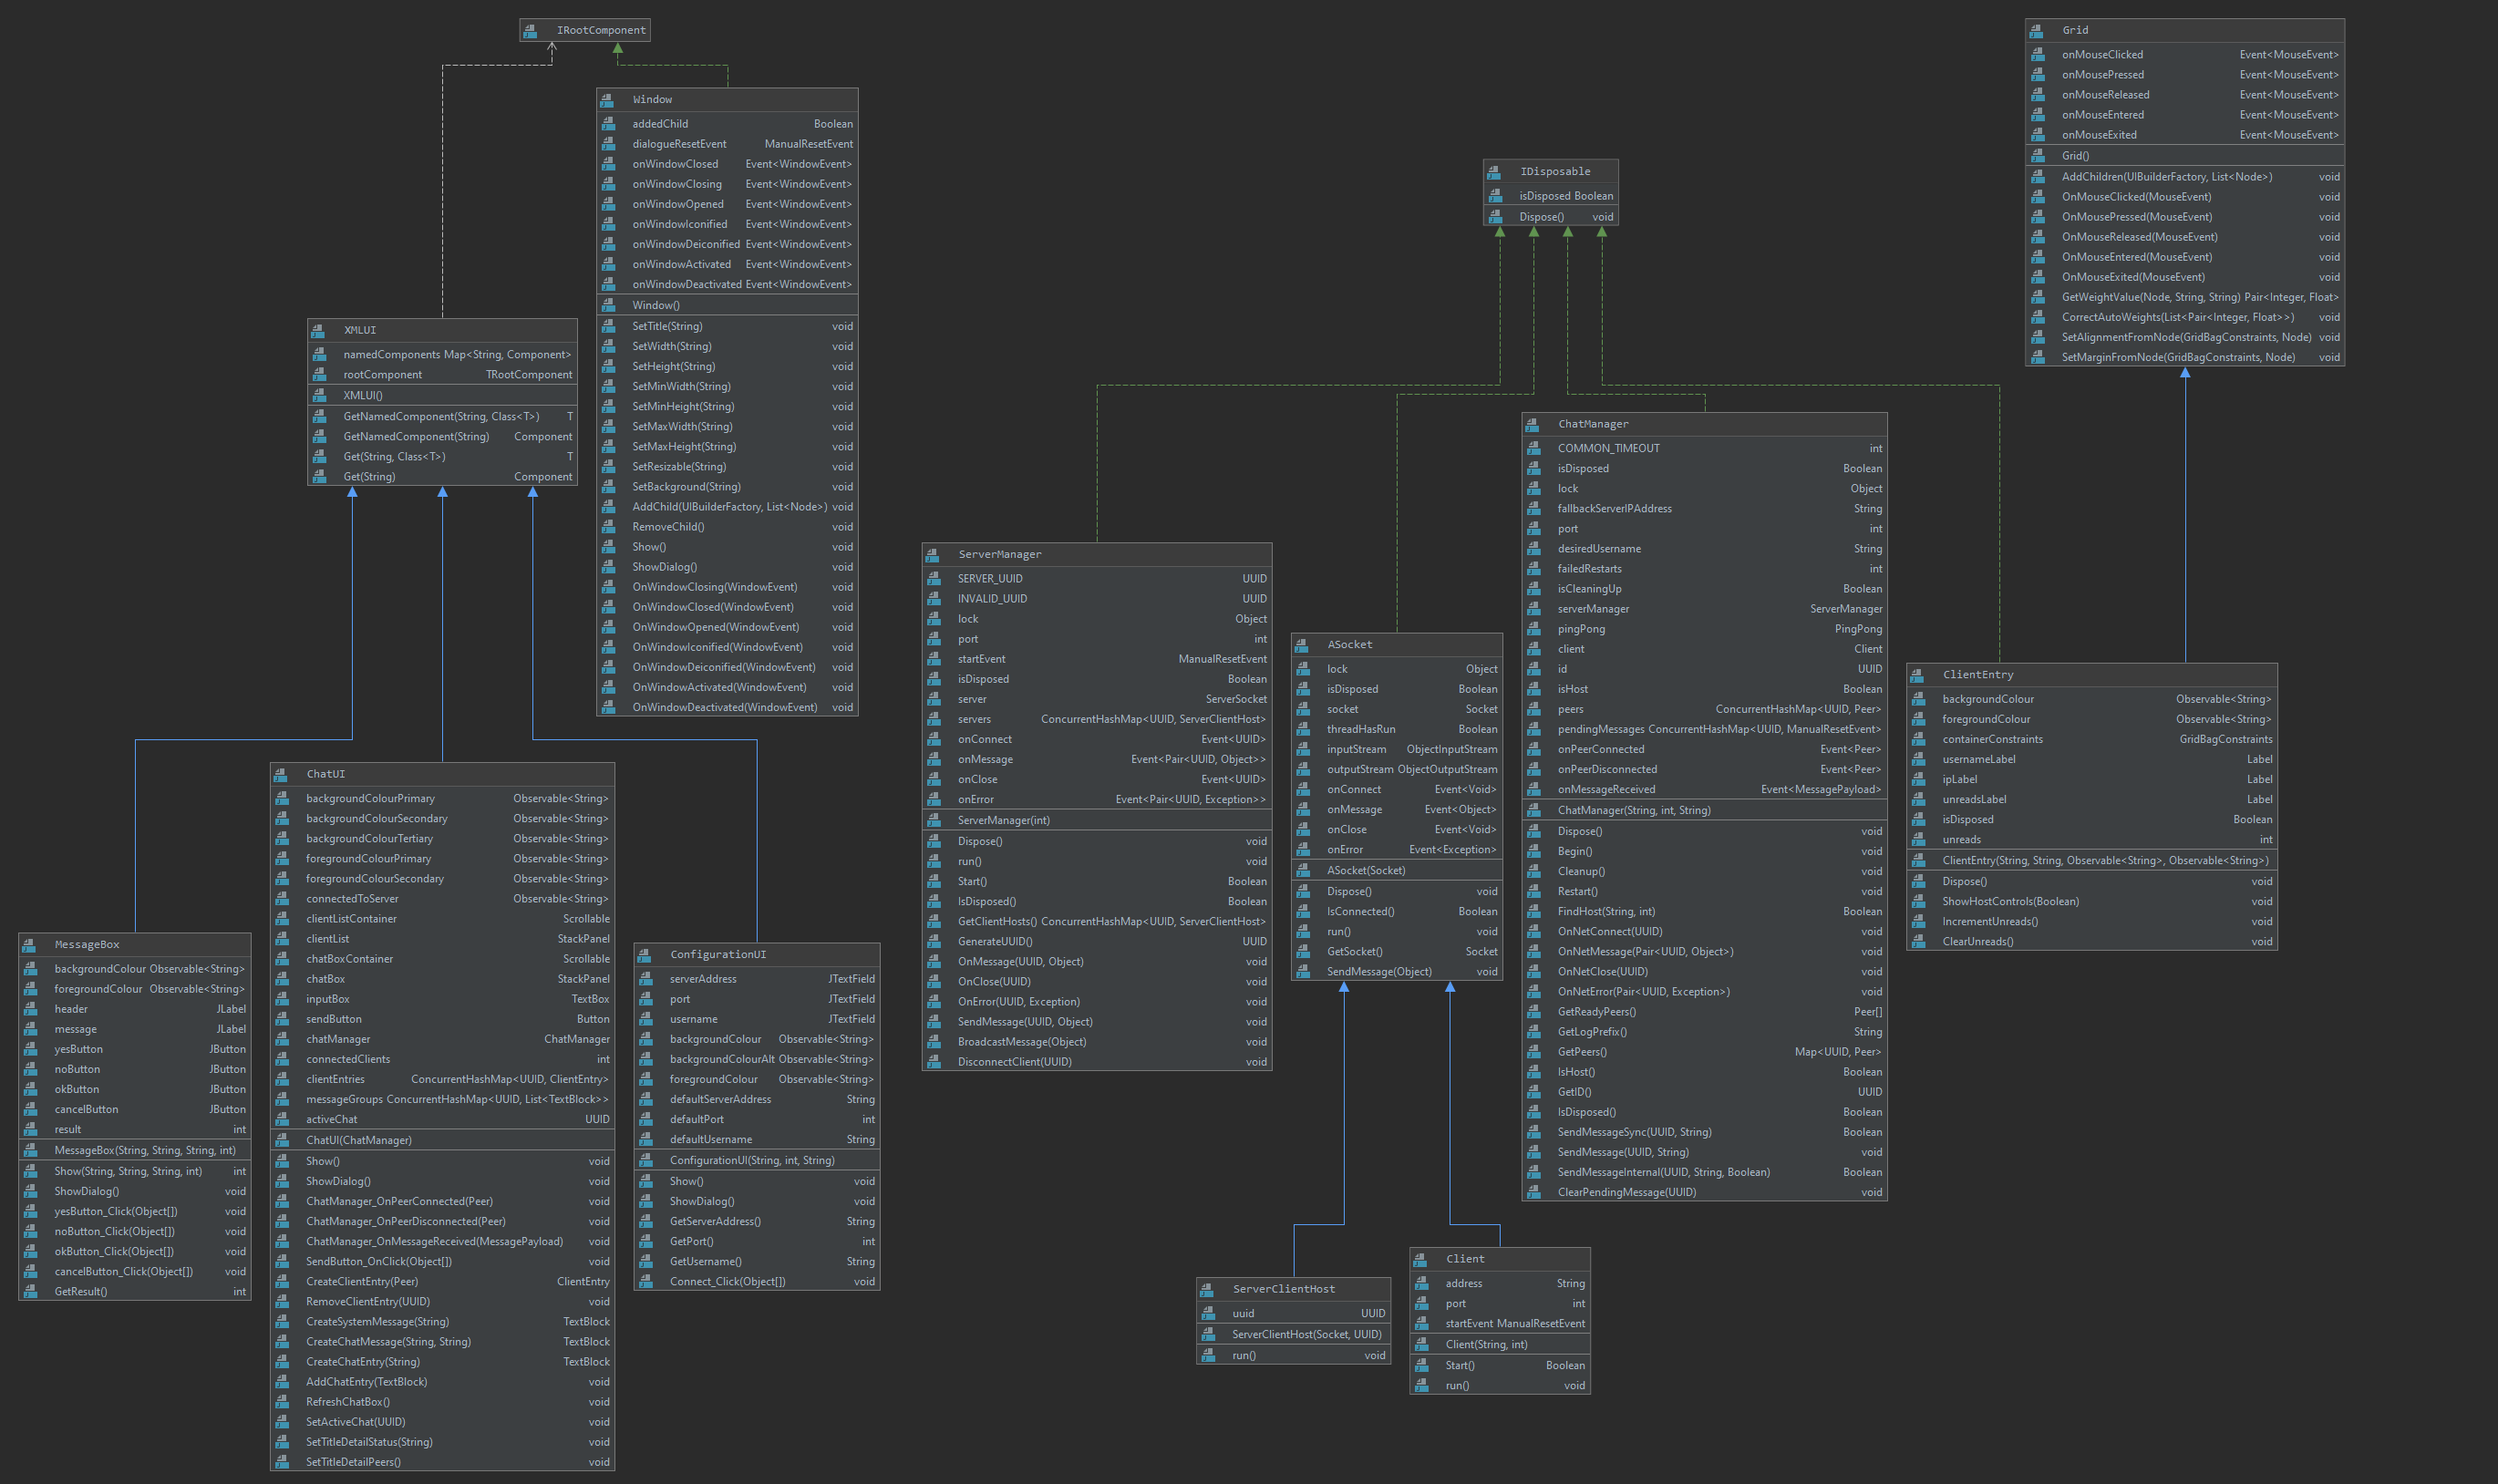
\includegraphics[width=0.5\textwidth]{uml.png}
\caption{UML Diagram}
\label{fig:figure1}
\end{figure}

\normalsize \textrm {Unit testing is important with projects as big as these as during development it is likely that many things will keep changing, and so we can make use of unit tests to make sure that parts of the program don't break when changes are made. We were originally going to create unit tests for the frontend (UI) by making use of the Windows Accessability API however Java Swing uses a custom renderer that is not compliant with the Windows UI framework, resulting is us not being able to use this approach for frontend (UI) tests. We were, however, able to make a five unit tests for the backend. Some of these tests include initializing the 'ChatManager' as a host or client, while others test if broadcast messaging works, if private messages only reach the intended recipient, and test the ping/pong timeout and the automatic host migration. These tests can be found in the 'src/testing' folder.\\
A simple test that we have written out will create two instances of the 'ChatManager' and verify that one instance starts up as a host and the other as a client. A more advanced test that we wrote tests if a private message is received by the intended recipient: this test creates three instances of the 'ChatManager' of which one will be the host and the other two will be clients. The test will then send a private message from one peer to another peer, and check that only the target peer received the private message.}

\normalsize \textrm {Our code made use of locks to prevent race conditions on network events as well as try/catch statements as certain exceptions would be raised for known network events, like when a peer disconnects. We don't want these exceptions to terminate the program so the are caught and handled accordingly.\\
While we have tried to keep the program as bug free as possible, it is almost always inevitable that bugs will be present in a program. For the most part, in the manual testing very few bugs have been experienced, however there is one that has been noticed that had no easy fix. Unfortunately, this bug is very difficult to reproduce, therefore making it equally as hard to fix. On rare occasions the bug occurs at startup when a client is trying to connect to a server. We are unsure as to what exactly is causing this issue, however we believe that it could be a race condition within the automatic migration system. This could also explain why the bug is so hard to reproduce. When looking at the error log and stack trace, the error seems to lie in parsing the data received which, after reading the error code online, is due to corrupt data \cite{streamcorruptedexception_invalid_type_code_ac}. This bug is a fatal bug to our project as it renders the entire application unusable and floods the console with this error indefinitely. Below in "Figure 2" you can see a screenshot of the error and the stack trace.}
\begin{figure}[h]
\centering
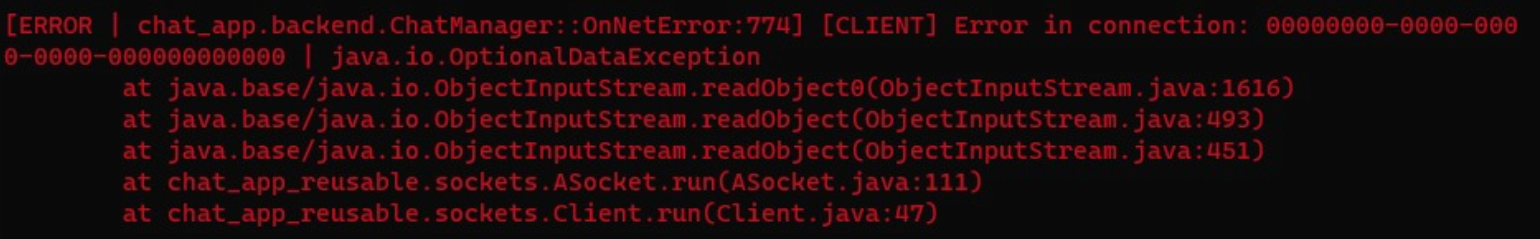
\includegraphics[width=0.5\textwidth]{rare_bug.png}
\caption{Rare Bug Screenshot}
\label{fig:figure2}
\end{figure}

\normalsize \textrm {Our addition of the XML UI builder made it easier to build and rapidly test new UI designs. In "Figure 3" we can see part of an XML file that is used to build the UI.}
\begin{figure}[h]
\centering
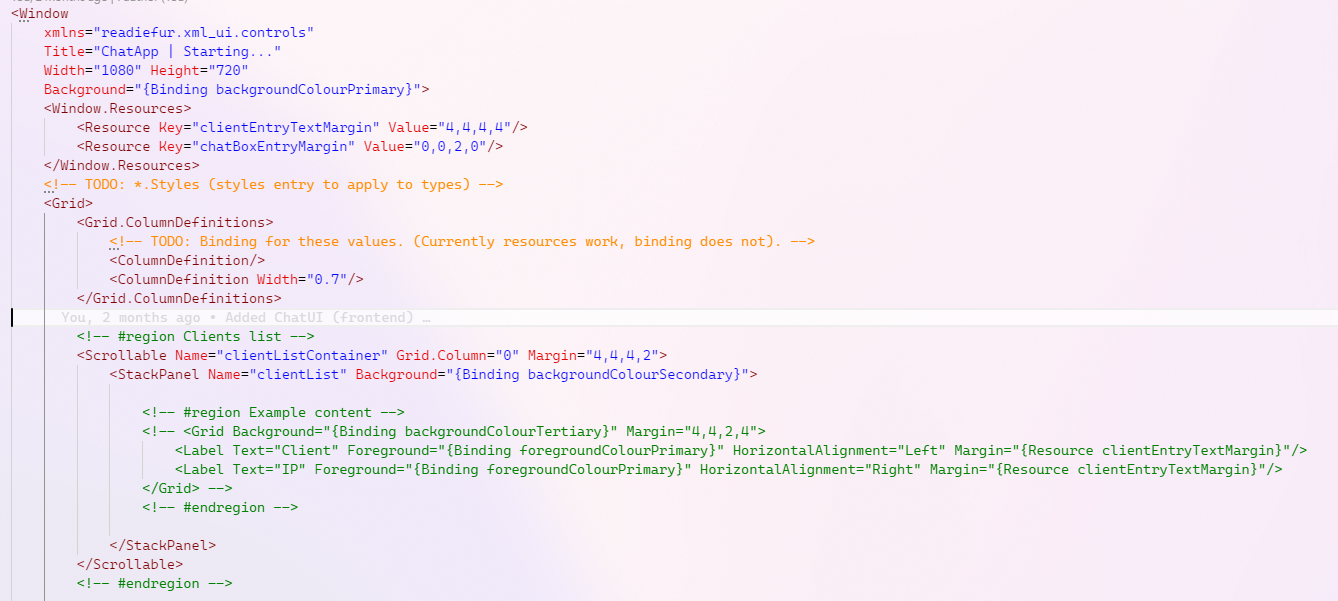
\includegraphics[width=0.5\textwidth]{xml_ui.png}
\caption{XML UI Screenshot}
\label{fig:figure3}
\end{figure}

\normalsize \textrm {If we focus on the commented out section, we can see a sample block of XML that would generate a peer entry on the UI. Because we needed this part of the UI to be dynamic and we didn't allow for non-root components to be loaded from XML, we had to create this UI element in code. Looking at the code in "Figure 4" below, it can be seen that the code is much more verbose and harder to read, as well as this only being part of the solution, therefore showing that the implementation of the XML UI builder was a good idea.}
\begin{figure}[h]
\centering
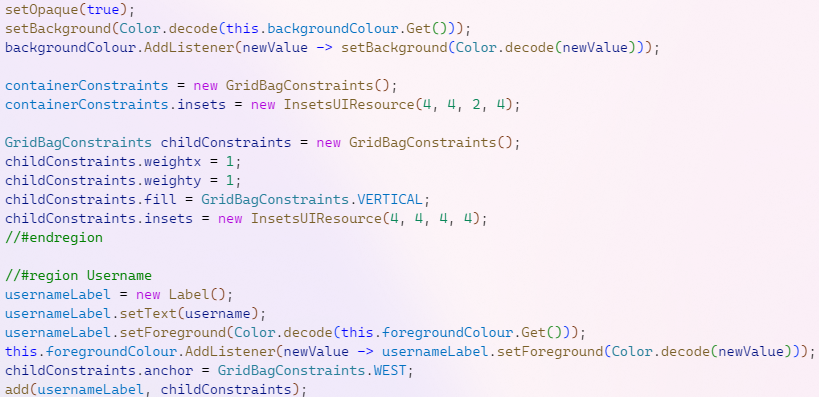
\includegraphics[width=0.5\textwidth]{code_ui.png}
\caption{Code UI Screenshot}
\label{fig:figure4}
\end{figure}

\section{IV. Conclusion}
\normalsize \textrm {Overall, we believe that the delivered project has been successful. There was only one major bug which only occurs on very rare occasions. We have enjoyed this coursework task and have managed to create a chat-app that has made use of many design patterns and features available to the Java programming language. As a group we were capable of sharing our knowledge and expertise within certain areas. We managed to successfully design, create and run the networked distributed system for a group-based client-server communication application, as well as create a simple yet effective Graphical User Interface. The chat application shows its practicality and value as it allows the users to communicate with each other on a functional and secure system, whereby a user-friendly graphical user interface makes it easier to utilize and operate.\\
The execution of the project would be enhanced if we were able to fix the bug and this is the obvious failing. However, as the failing is rare and difficult to recreate we have not been able to address this as we would have liked. Overall, however, we are pleased with the other learning, developments and features created. }

% \bibliographystyle{agsm}
% \bibliography{references.bib}
% The above auto-bibliography for the references didn't seem to be working so I will try my best to manually format the references below.

\begin{thebibliography}{9} % Replace "9" with the number of references you have

\bibitem{buildyourownCommandLinewithANSIescapecodes}
Haoyi (2023) \textit{Build your own Command Line with ANSI escape codes}.

\bibitem{convert_a_number_range_to_another_range_maintaining_ratio}
Jerryjvl (2023) \textit{Convert a number range to another range, maintaining ratio}.

\bibitem{csharptools_pipes}
ReadieFur (2023) \textit{CSharpTools.Pipes}.

\bibitem{streamcorruptedexception_invalid_type_code_ac}
User207421 (2023) \textit{StreamCorruptedException: invalid type code: AC}.

\bibitem{windowlistener}
Oracle (2023) \textit{WindowListener}.

\end{thebibliography}

\end{document}
